\documentclass[a4paper,11pt]{article}

\usepackage[utf8]{inputenc}
\usepackage{mathtools}
\usepackage{hyperref}
\usepackage{units}
\usepackage[spanish]{babel}
\usepackage{graphicx}

\title{Probabilidad multidimensional}
\author{Análisis Estadístico de Datos}
\date{}

\pdfinfo{
  /Title    (Probabilidad multidimensional)
  /Author   (Diego Ravignani)
  /Creator  ()
  /Producer ()
  /Subject  (Análisis Estadístico de Datos)
  /Keywords ()
}

\begin{document}
\maketitle

\begin{enumerate}


\item Graficar las superficies de nivel 1$\sigma$ de las distribuciones binormales con parámetros $\mu_1 = 1.3$, $\mu_2 = 0.5$, $\sigma_1 = 1.7$, y $\sigma_2 = 2.3$ para tres diferentes correlaciones $\rho = -0.9$, $0$ y $0.5$. 



\item Considerar dos variables independientes $X_1$ y $X_2$ distribuidas con la función de densidad de probabilidad binormal,

$$ f(x_1,x_2) = \frac{1}{2 \pi \sigma_1 \sigma_2} \, \mathrm{exp} \bigg(- \frac{q(x_1,x_2)}{2}  \bigg), $$ 

\noindent dónde $$ q(x_1,x_2) = \left(\frac{x_1-\mu_1}{\sigma_1}\right)^2  + \left(\frac{x_2-\mu_2}{\sigma_2}\right)^2 .$$ 

Transformar a una variable $\chi^2$ para calcular la probabilidad que la variable aleatoria bidimensional ($X_1$, $X_2$) caiga en las regiones 1$\sigma$, 2$\sigma$ y 3$\sigma$ definidas por las elipses $q = 1$, $q = 4$ y $q = 9$ respectivamente.
Sin hacer cuentas, pensar como cambiarían las elipses si $X_1$ y $X_2$ estuvieran correlacionadas y cuánta probabilidad contienen las elipses 1$\sigma$, 2$\sigma$ y 3$\sigma$.


\item Considerar una variable aleatoria normal bivariada con parámetros $\mu_1 = \mu_2 = 0$, $\sigma_1 = \sigma_2 = 1$ y correlación $\rho \ne 0$. Escribir la matriz Hessiana $\boldsymbol{A}$ co\-rres\-pondiente a estos cinco parámetros y encontrar analíticamente sus autovalores y autovectores. Graficar las regiones 1$\sigma$, 2$\sigma$ y 3$\sigma$ correspondientes a la forma cuadrática $q(\boldsymbol{x}) =  \boldsymbol{x}^T \boldsymbol{A} \boldsymbol{x}$  para $\rho = -0.9$.


\item Mostrar que la elipse 1$\sigma$ de una variable normal bivariada $(X_1, X_2)$ con parámetros  $\mu_1$, $\mu_2$, $\sigma_1$, $\sigma_2$ y $\rho$ está circunscripta dentro de un rectángulo de semiancho $\sigma_1$ en el eje $X_1$ y  $\sigma_2$ en el eje $X_2$ como muestra la figura \ref{fig:1sigma}.

\begin{figure}[h]
 \begin{center}
 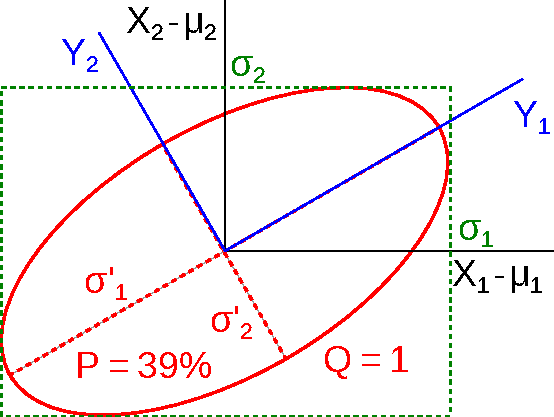
\includegraphics[scale=0.6]{elipse_1sigma}
 % elipse_1sigma.pdf: 0x0 px, 300dpi, 0.00x0.00 cm, bb=
\end{center}

\caption{Rectángulo circunscripto en la elipse 1$\sigma$. \label{fig:1sigma}}
\end{figure} 

% Cambio de coordenadas polares
\item Considerar una variable normal bivariada con medias $\mu_1$ y $\mu_2$, desviaciones estándares $\sigma_1$ y $\sigma_2$ y coeficiente de correlación $\rho$. El cambio a coordenadas polares $r$ y $\theta$ es tal que su inversa es,

$$
T^{-1}: (r, \theta) \rightarrow (x_1, x_2 ) 
\begin{cases}
x_1 = \mu_1 + r \, \sigma_1 \, \cos\theta \\
x_2 = \mu_2 + r \, \sigma_2 \, \sin\theta \\
\end{cases}
$$


\noident Aplicando el cambio de variables correspondiente, calcular la función de densidad de probabilidad conjunta de $r$ y $\theta$. En base a esta PDF decidir si $r$ y $\theta$ son variables aleatorias independientes o no. Calcular las PDF marginales de $r$ y $\theta$. 

% En base a la PDF marginal de $r$, calcular la PDF de $u = r^2$ y comparar con la PDF de una variable chi-cuadrado con dos grados de libertad.   

% Propagación de la varianza
\item La eficacia de una vacuna (VE) se puede medir en un test clínico en base a la proporción de pacientes contagiados vacunados con respecto al número total de pacientes contagiados ($p$), 

$$ \mathrm{VE} = \frac{1-2\,p}{1-p}$$. 

En el test de la vacuna covid de Astra-Zeneca se estimó que la media de la variable aleatoria $p$ es $\mathrm{E}(p) = 0.28$ y su desviación estándar es $\sigma(p) = 0.05$. Aplicando la fórmula de propagación de la varianza calcular la media y la desviación estándar de la eficacia VE. 


% \item Consider the random variables $x_1$ and $x_2$ and their sum $y = x_1 + x_2$. Calculate the variance of the random variable $y$ in terms of the variances and covariance of $x_1$ and $x_2$. What is the variance of $y$ in the special case $x_1 = x_2$? How does the result change if $x_1$ and $x_2$ are independent  identically distributed (iid) variables? 

\item Considerar dos variables independientes $X_1$ y $X_2$ con varianzas $\sigma_1^2$ y $\sigma_2^2$. 
Calcular la matriz de covarianza de las nuevas variables $Y_1 = X_1 + X_2$ y $Y_2 = X_1 - X_2$ en términos de $\sigma_1$ y $\sigma_2$. Calcular la correlación entre $Y_1$ e $Y_2$ y decidir si estas dos variables son independientes o no.

% \item Consider the vector variable $\boldsymbol{x}$ in m~dimensions and $\boldsymbol{y} = \boldsymbol{B} \boldsymbol{x}$ in n~dimensions. Calculate the covariance matrix of $\boldsymbol{y}$ in terms of the covariance matrix of $\boldsymbol{x}$. 




% Regresión lineal como combinación lineal de una variable normal multidimensional

\item  En un experimento se miden los siguientes datos que se ajustan con una regresión lineal: 

\begin{center}
    \begin{tabular}{crr}
    i & $x_i$ & $y_i$ \\ \hline
    1 & 1 & 1.85 \\
    2 & 2.5 & 2.72 \\
    3 & 3.1 & 5.15 \\
    4 & 4 & 5.7 \\
    5 & 5.5 & 6.9 
    \end{tabular} 
\end{center} 

Los datos $y_i$ se consideran como un vector $\boldsymbol{y}$ de cinco variables normales. 
Se asume además las variables $y_i$ tienen la misma desviación estándar $\sigma = 0.5$ (homocedasticidad). 
La pendiente ($\hat{m}$) y la ordenada al origen ($\hat{y}_0$) de la recta que ajusta los datos son una nueva variable aleatoria de dos dimensiones: 

$$ \boldsymbol{\hat{\theta}} = 
\begin{pmatrix}
\hat{y}_0 \\
\hat{m} \\
\end{pmatrix} $$

Sus valores se calculan con la multiplicación de matrices $\boldsymbol{\hat{\theta}} = \mathbf{B} \, \boldsymbol{y}$ dónde
 $$
 \boldsymbol{B} = 
\begin{pmatrix}
0.834  &    0.406  &    0.234  &   -0.023  &   -0.451 \\
 -0.197  &    -0.064  &  -0.011 &    0.069  &    0.202 \\
 \end{pmatrix}
 $$.

Calcular la ordenada al origen y la pendiente de la recta que ajusta los datos. Graficar los datos y el ajuste.
Expresar la matriz de covarianza de $\boldsymbol{y}$. Considerando que la variable aleatoria en dos dimensiones $\boldsymbol{\hat{\theta}}$ es una combinación linear de la variable aleatoria en cinco dimensiones $\boldsymbol{y}$ vía la matriz $\boldsymbol{B}$, calcular la matriz de covarianza de $\boldsymbol{\hat{\theta}}$. Calcular las desviaciones estándares de  $\hat{y}_0$, $\hat{m}$ y su correlación. Identificar la distribución que sigue $\boldsymbol{\hat{\theta}}$ y los valores de sus parámetros. 
 

%\item Considerar la variable Gaussiana $x$ distribuída con parámetros $\mu=5.7$ y $\sigma=1.3$. Con la fórmula de propagación de la variancia estimar la variancia de la nueva variable $y=x^2$. Calcular aparte la variancia exacta de la variable $y$ considerando que $\mathrm{Var}(x^2)= \mathrm{E} \left( \left[ x^2 - \mathrm{E}(x^2) \right]^2 \right)$. Usar que el momento de segundo orden de $x$ es $\mathrm{E}(x^2)=\mu^2+\sigma^2$ y el de cuarto orden  $\mathrm{E}(x^4)=\mu^4+6\mu^2\sigma^2+3\sigma^4$. Comparar la variancia exacta con la estimada a partir de la propagación de la varianza.

% Change of variables
% \item Consider the random vector $\boldsymbol{x}$ in 2 dimensions and the change to polar coordinates $ r^2 = x_1^2 + x̣_2^2$ and $\theta = \tan \left( x_1/x_2 \right)$. Calculate the probability distribution function $f(r,\theta)$ given that $\boldsymbol{x}$ follows a standard binormal distribution and that $x_1$ and $x_2$ are independent. Calculate the marginal PDF $g(r)$ and the PDF of $r^2$.  

% Calculo de la distribución condicional de una binormal => lo saco, muchas cuentas...
% Consider a generic binormal distribution with parameters $\mu_1$, $\mu_2$, $\sigma_1$, $\sigma_2$, and correlation $\rho$. From the joint distribution $f(x_1, x_2)$ and the marginal distribution $g_1(x_1)$ show that the condition distribution $h(x_2|x_1)$ is a Gaussian with parameters $\mu' = \mu_2 + \rho \, \frac{\sigma_2}{\sigma_1} (x_1 - \mu_1)$ and $\sigma'^2= \sigma_2^2 \, (1-\rho^2)$. If $x_1$ is positive, what is the sign of the most probable values of $x_2$ if the correlation is positive or negative? 

% Change of variables
% \item mostrar que $\lambda_1 \, \lambda_2 = \frac{1}{{\sigma_1^2 \sigma_2^2 (1-\rho^2)}$

\end{enumerate}

\end{document}
